\section{Data}
\label{sec:data}

We explore the behavior of the metrics on mock classifications with well-understood weaknesses as well as realistic mock classifications from past challenges.
Data is in the form of catalogs of posterior probability vectors $p(m \mid d)$ over $M$ classes $m$ conditioned on the observed lightcurve $d$, with each probability vector normalized to sum to unity.\footnote{Throughout the paper, ```data'' always refers to classification results, not lightcurves; no \plasticc\ lightcurves were simulated, viewed, or classified in the preparation of \textit{this} paper.}
% We introduce the convention that the $M^{\mathrm{th}}$ class is designated ``other'' to encompass never-before-seen classes.
We introduce the confusion matrix $\mathbb{C}$, an $M\times M$ dimensional table of empirical probabilities $p(m \mid m')$ traditionally calculated from deterministic classification point estimates with knowledge of the true classes $m'$.
% TODO define TP/FP/TN/FN here
Though probabilistic classifications are not truly compatible with the confusion matrix, we use it as a middle ground to develop intuition from conceptually familiar deterministic classifications.

\subsection{Mock classifications}
\label{sec:mockdata}

The test cases of this section are devised to confirm that our metric aligns with our intuitive understanding of what constitutes a good classifier, that it should not reward classifications suffering from the most concerning error properties, which we will refer to as \textit{systematics} throughout the paper.
We consider a situation with $M=13$ classes
% (nominally $12$ with one designated as ``other,'' meaning not represe) and
with a lognormal distribution of the number $N_{m}$ of members of each class.

We present eight mock classifiers whose systematics are encapsulated by their confusion matrix $\mathbb{C}$.
Each classifier derives classification posteriors $p(m \mid m')$ based on the true classes as a proxy for the information contained in the lightcurves, which we hope to recover.
The posterior probability vector for a given object is a perturbation of the row of the confusion matrix corresponding to its true class, with a perturbation factor of $\delta=0.1$, following
\begin{eqnarray}
  \label{eq:cmtoprob}
  p(m \mid m') &=& \mathbb{C}_{m'} + \delta\vec{\epsilon},
\end{eqnarray}
where the perturbation vector $\vec{\epsilon}$ has components drawn from a half-Cauchy distribution
\begin{eqnarray}
  \label{eq:cauchy}
  f(x) &=& \frac{2}{\delta\pi} \left(1+\left(\frac{x+x_{0}}{\delta}\right)^{2}\right)^{-1}
\end{eqnarray}
with $x_{0}=0$.
% \aim{[Rahul: Might be good to have a plot of the pdf when x0 takes values close to 0., something like 0.4, 0.8 and close to 1.0]}

% TODO: sequential color scheme?
% TODO: letters for panels, refer to them in text

\begin{figure*}
	\begin{center}
    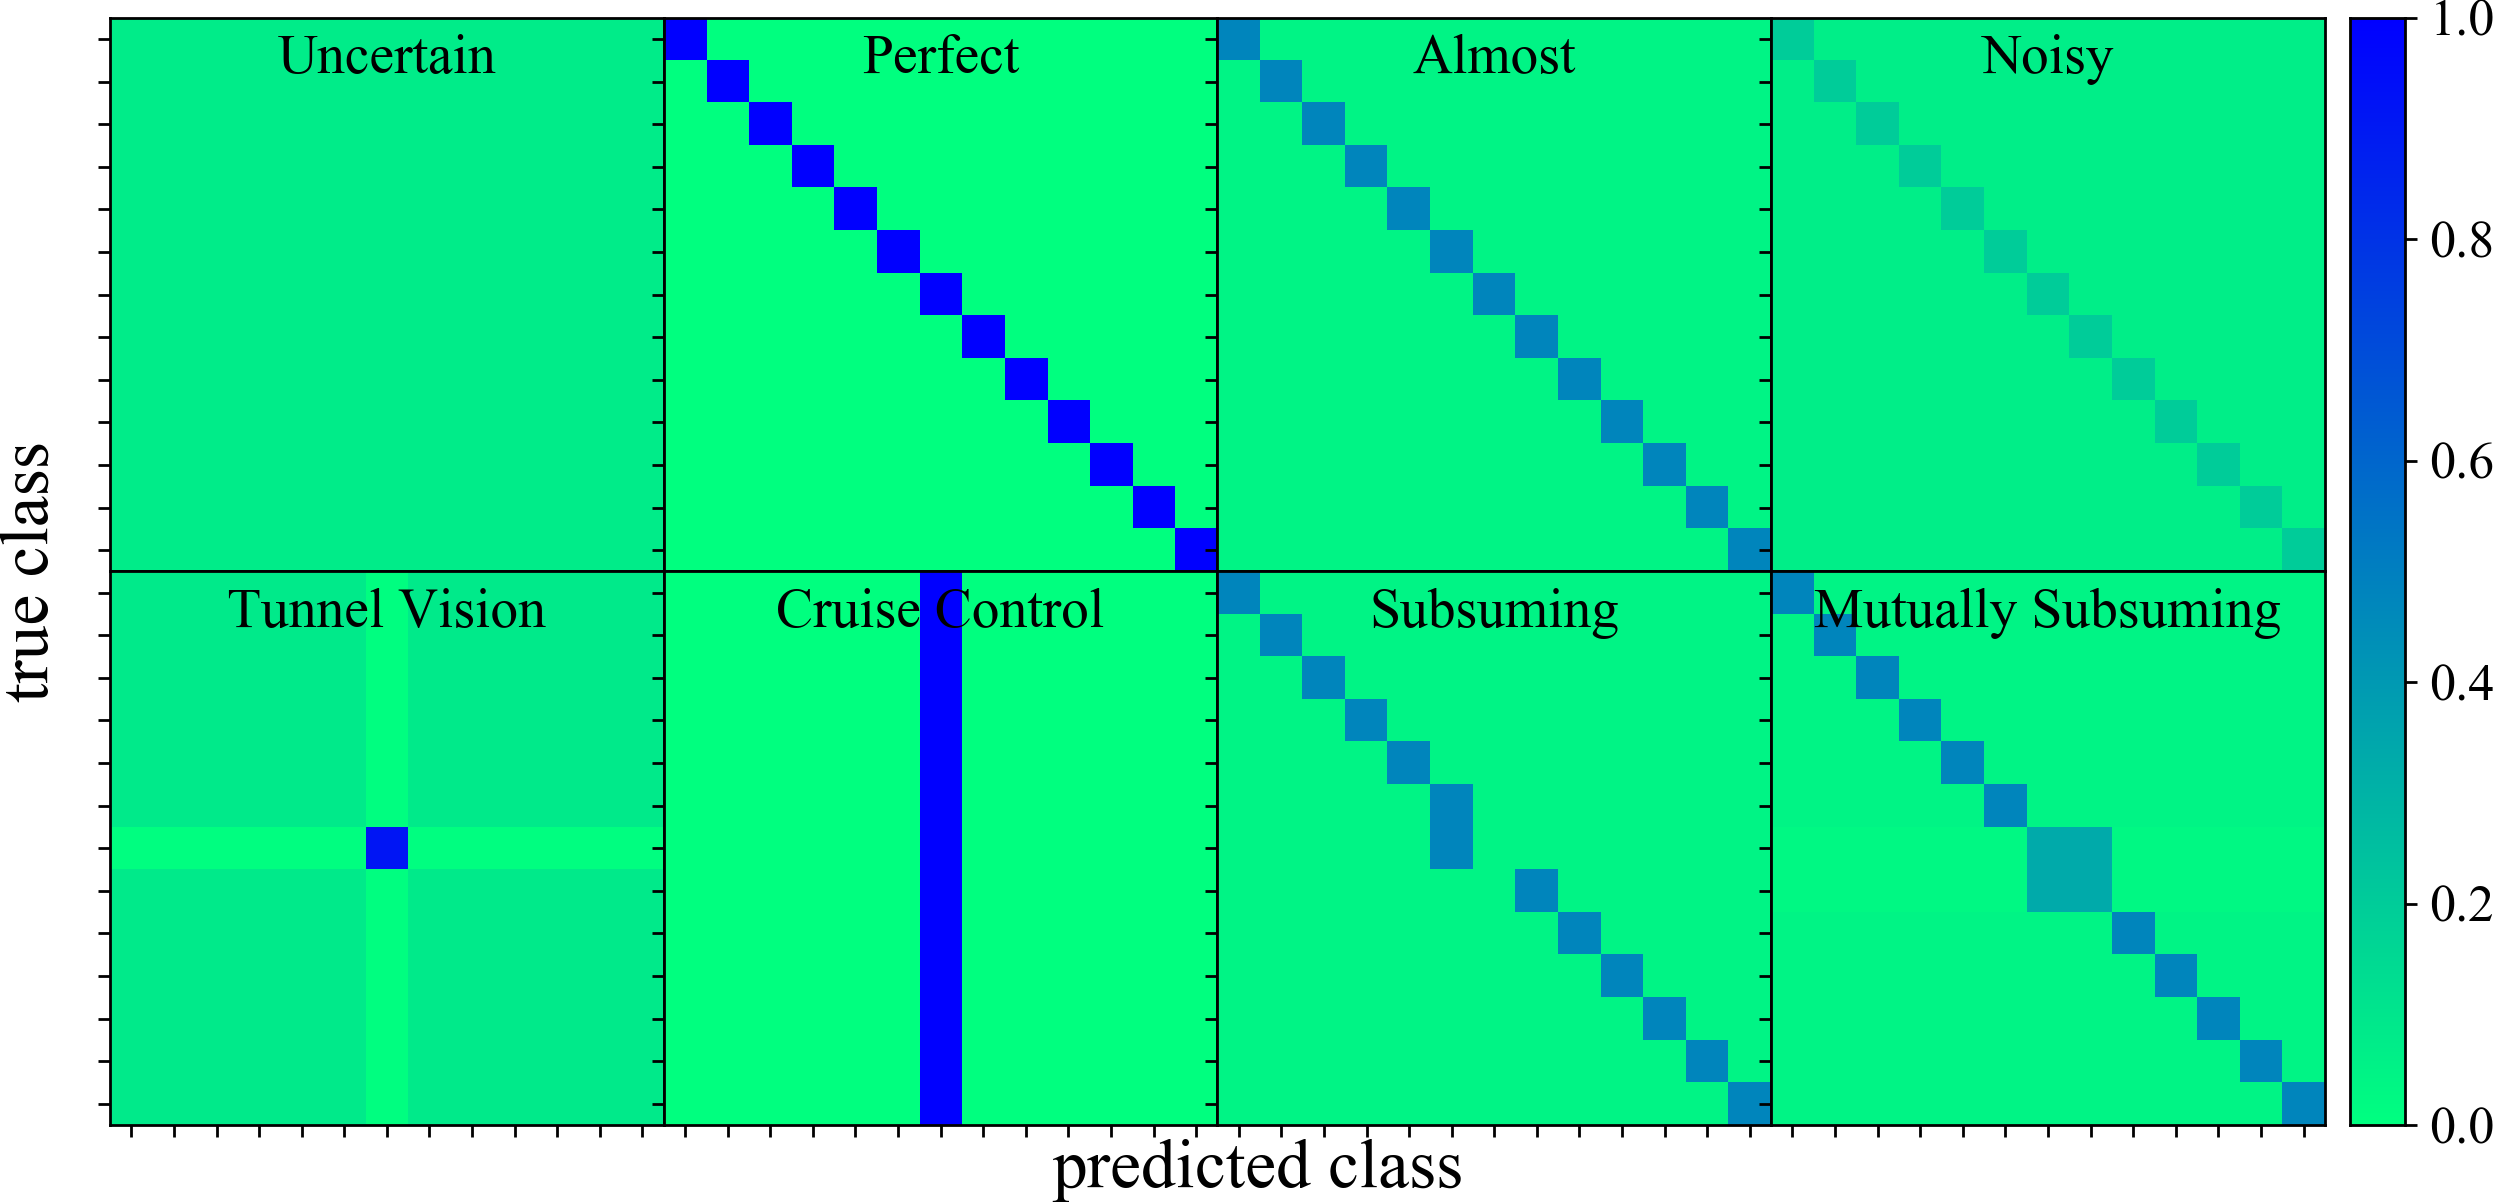
\includegraphics[width=0.8\textwidth]{./fig/all_sim_cm.png}
		\caption{Confusion matrices for eight mock classifiers.
    leftmost top: uncertain classification,
    leftmost bottom: perfect classifications,
    left-center top: almost perfect classification,
    left-center bottom: unbiased classifications,
    right-center top: perfect classification (type 1 and type 2 errors) for one class and uniform for all others,
    right-center bottom: assigning all objects the same class,
    rightmost top: consistently assign one class to another,
    rightmost bottom: consistently assign another class to one class}
		\label{fig:mock_cm}
	\end{center}
\end{figure*}

Figure~\ref{fig:mock_cm} shows the confusion matrices corresponding to each systematic considered, discussed in detail below.
For each case, we address:
\begin{enumerate}
  \item What defines this error property?
  \item Under what conditions is this error property relevant?
  \item What are our expectations and desires for this error property's effect on metric behavior?
\end{enumerate}

\subsubsection{Uncertain classification}
\label{sec:uncertaindata}

An entirely uniform confusion matrix $\mathbb{U}$ (leftmost top panel of Figure~\ref{fig:mock_cm}) would correspond to uniform random guesses for deterministic classification, but the probability vectors drawn from it are more nuanced.
In accordance with Equation~\ref{eq:cmtoprob}, the probability vectors are perturbations away from a uniform distribution across all classes.
The peak values of these probability vectors will correspond to uniform random classifications, however, with $p(m' \mid d)\approx M^{-1}$.
We can consider the \textit{uncertain} classifier as an experimental control for the worst possible classifier, noting that if classifications were anticorrelated with true classes, the experimenter would simply relabel them to improve performance.

\subsubsection{Accurate classification}
\label{sec:accuratedata}

The \textit{perfect} classifier has a diagonal confusion matrix $\mathbb{I}$ (leftmost bottom panel of Figure~\ref{fig:mock_cm}), which would correspond to deterministic classifications that are always correct.
In terms of probabilistic classifications, a perfect result would be a probability vector with 1 for the true class and 0 for all other classes.
Due to our addition of the random perturbation factor $\vec{e}$, the probability vectors drawn from the perfectly diagonal confusion matrix are randomly perturbed away from perfect classifications by the small factor $\delta$, but the class with maximum probability is almost always still the true class, to the tune of $\sim0.96$ with our choice of $\delta$.
This case is also a control, in that \plasticc\ would not be necessary if we believed the perfect classifier were realistically achievable.

In addition to a perfect classifier, we test linear combinations
\begin{eqnarray}
  \label{eq:lincomb}
  \mathbb{C}^{\mathrm{acc}; s} &=& \frac{1}{M+s-1} \left(s\mathbb{I} + \mathbb{U}\right)
\end{eqnarray}
of the perfect and uncertain classifier confusion matrices where the contribution of the perfect classifier is greater that of the uncertain classifier by a factor of $s$.
Deterministic classifications drawn from such a confusion matrix would be correct $s$ times as often as they are wrong, and the incorrect guesses would be uncorrelated across classes.
The probability vectors drawn from such confusion matrices would have some variability but still mostly have their peak value at the truth.
We consider the case of the \textit{almost perfect} classifier with $s=4$ (left-center top panel of Figure~\ref{fig:mock_cm}) and the \textit{noisy} classifier with $s=2$ (left-center bottom panel of Figure~\ref{fig:mock_cm}), which correspond to $p(m' \mid d)\approx0.82$ and $p(m' \mid d)\approx0.62$ respectively.
We expect that the response to variation in $s$ may differ across metrics.
(Though $s$ would realistically be expected to vary for each class, we do not conduct a systematic investigation of this possibility at this time.)

A classifier with different accuracy for each class may be considered a systematic in its own right.
An extreme example of such a classifier could be one with perfect classification performance on one class and uncertain classification on all others; its confusion matrix would be uniform except for one row, which would take a value of unity on the diagonal and zero elsewhere.
Such a classifier would have high value to those who study the class with perfect performance and should still be used in the context of \lsst.
However favoritism is inappropriate for the overall \plasticc\ metric, which must serve the needs of those who study all the classes and for different purposes.
From the perspective of \plasticc, such a \textit{tunnel vision} classifier (right-center panel of Figure~\ref{fig:mock_cm}) is a major concern.

\subsection{Inaccurate classification}
\label{sec:inaccuratedata}

Inaccurate classification in the context of a deterministic classifier is self-explanatory.
If a classifier is \textit{systematically} inaccurate, its confusion matrix has significant probability on off-diagonal elements.
We model inaccurate probabilistic classifications of class $m'$ by using the row of the confusion matrix corresponding to class $\tilde{m}$ as the basis for the perturbed probability vector
\begin{eqnarray}
  \label{eq:subsume}
  p(m\ \mid\ m') = p(m\ \mid\ \tilde{m}).
\end{eqnarray}
Class $m'$ is said to be \textit{subsumed} by class $\tilde{m}$ for such a classifier.
The asymmetric relationship between $m'$ and $\tilde{m}$ is illustrated in the rightmost top and bottom panels of Figure~\ref{fig:mock_cm}.

It is possible that the \plasticc\ classes will be subtypes of broader classes, as identifying classifiers that can distinguish between subtypes is especially relevant when the subtypes have wholly different science applications.
For example, SN Ia and SN Ibc are challenging to distinguish, and the former often subsumes the latter, an effect that can be exacerbated by underrepresentation of SN Ibc in available training sets.
However, using SN Ibc in the traditional cosmology analysis done with SN Ia can bias estimates of the cosmological parameters, so the distinction is critical.
We would like the \plasticc\ metric to identify the strength of a classifier that successfully prevents this error.

An extreme case of inaccurate classification is to classify all objects as the most common class, a particular concern for \plasticc\ given the potential for population imbalance between classes.
For our purposes, it matters not whether the subsuming class is actually the most common or only the most common in the training set.
Such a \textit{cruise control} classifier (right-center bottom panel of Figure~\ref{fig:mock_cm}) could be especially detrimental to \plasticc's goal of identifying objects belonging to extremely rare classes, particularly if the metric weights all objects equally.
Though we defend against this systematic by employing per-class weights, described in Section~\ref{sec:weights}, we nonetheless examine its impact under other plausible weighting schemes.

% \subsubsection{Combination of systematics}
% \label{sec:combo}
%
% \begin{figure}
% 	\begin{center}
% 		% 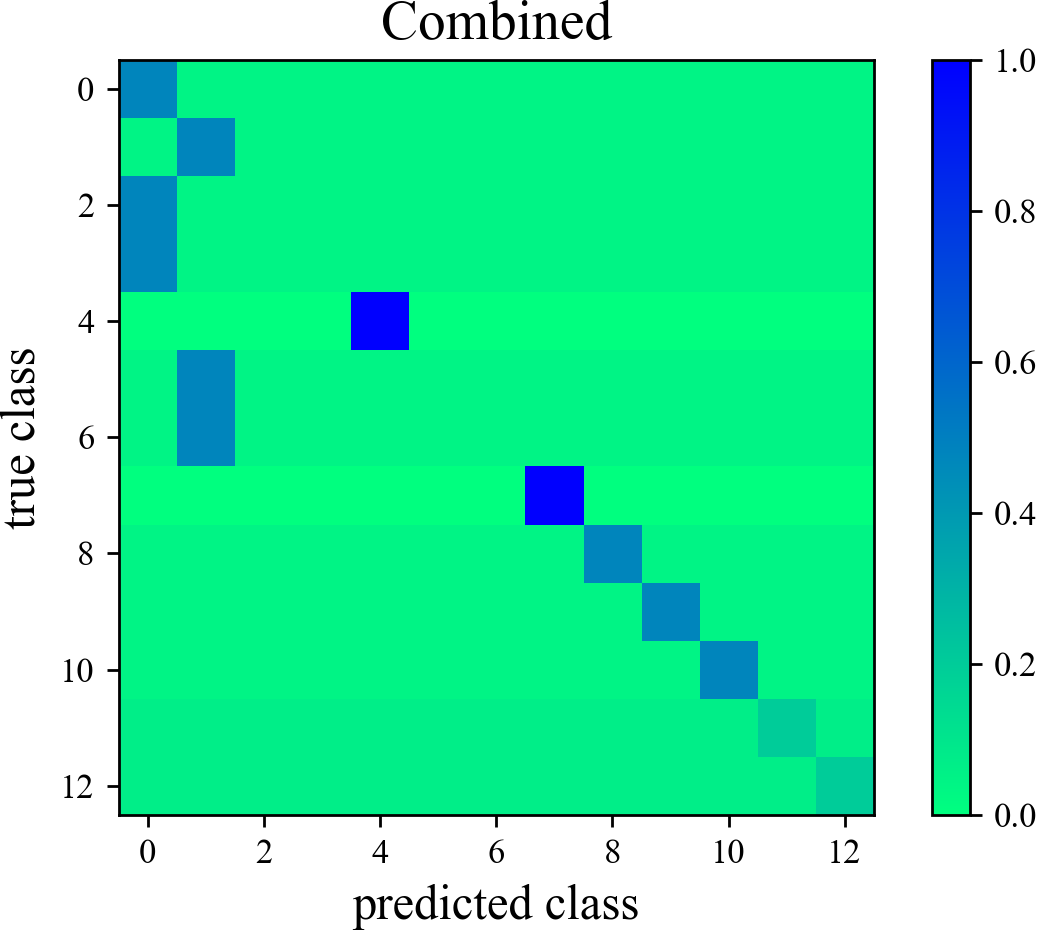
\includegraphics[width=0.45\textwidth]{./fig/Combined.png}
% 		\caption{}
% 		\label{fig:combo_cm}
% 	\end{center}
% \end{figure}

\subsection{Representative classifications}
\label{sec:realdata}
%\aim{This would be more meaningful if we were given the confusion matrices of actual submissions to \snphotcc\ and then checked whether the \plasticc\ metric would have designated a different winner.
%Also, it may be more interpretable if we instead use Ashish's confusion matrices that have more classes.}

\snphotcc\ \citep{kessler_supernova_2010} focused on separating the lightcurves of a heterogenous population into a limited number of subclasses, with a goal of identifying one particular type of object for a single scientific application, and attracted diverse classification approaches, including $\chi^{2}$ fits of the SN data to publicly available templates \citep{2002PASP..114..803N} physical models \citep{2008ApJ...681..482C}, and empirical models as well as alternatives to curve-fitting such as
%, and a linear slope to magnitudes per day was used for the non-Ia sample.
outier identification on the training set Hubble diagram, dimensionality reduction,
% TODO cite InCA?
and clustering.
% A general light curve shape (rather than one motivated by the physical differences between SNeIa and core collapse SNe) was assumed by some competitors and then a kernel density estimation was performed over the fit parameters, with various approaches employed including boosting over the feature space.
Machine learning was also employed over features such as the light-curve slopes to produce a predictive model for the training data.
For more information on these methods and their success within the \snphotcc, we refer the reader to \cite{kessler_results_2010}.
In short, \snphotcc\ attracted physically motivated template-based methods sensitive to the differences between the test data and the template set
%, which are prone to bias given non-representativity of the test data and agnostic
as well as those based on decomposition of the light curves into generic features at risk of neglecting available physical information.


After the \snphotcc\ concluded, the lightcurves became a testbed for a suite of machine learning classifiers.
We consider one such compilation of methods, as presented in \cite{lochner_photometric_2016}, whose confusion matrices are shown in Figure~\ref{fig:snphotcc_cm}.
These classification algorithms include a wavelet decomposition of the spectra to construct the features over which to classify (\citet{2011MNRAS.414.1987N}, bottom row) and template-based classification procedures (\citet{2011ApJ...738..162S}, top row), each paired with Boosted Random Forest, K-Nearest Neighbors, Naive Bayes, Support Vector Machine, and Neural Network machine learning algorithms (columns).
While the complexity of entries to the \snphotcc\ was greater than this subset, we use these illustrative examples as a useful comparison set over which to assess the performance of the approaches under our metric scheme.

\begin{figure*}
	\begin{center}
    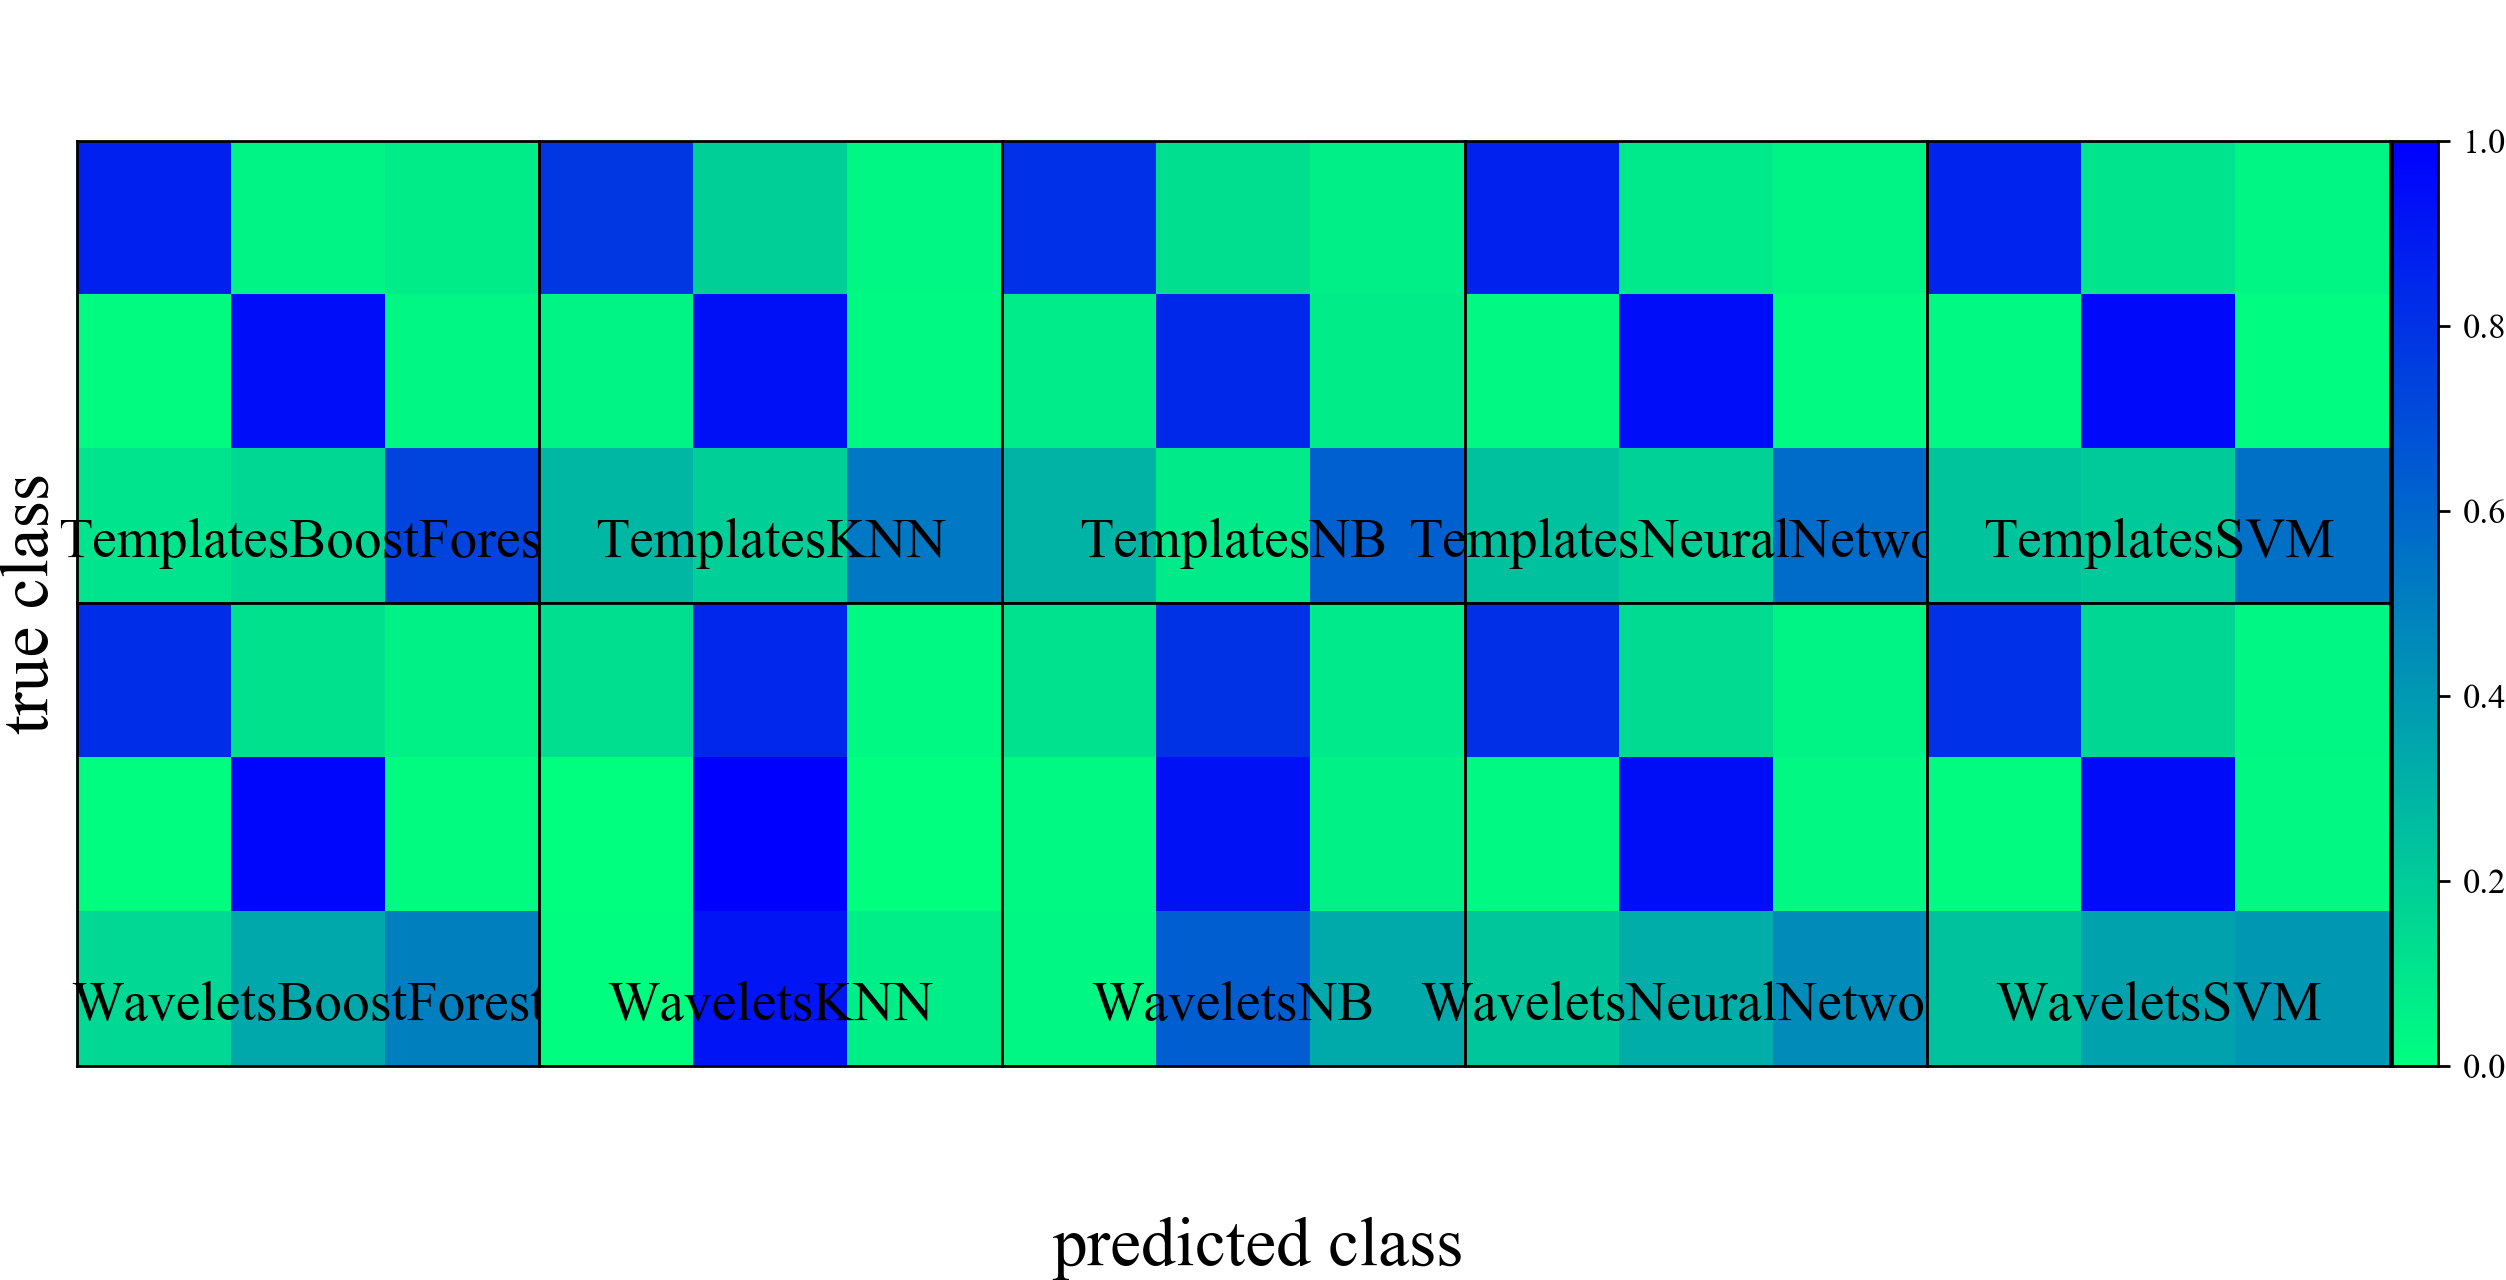
\includegraphics[width=\textwidth]{./fig/all_snphotcc_cm.png}
		\caption{\snphotcc\ confusion matrices.
    Top row: five machine learning methods applied to template decompositions.
    Bottom row: the same five machine learning methods applied to wavelet features.}
		\label{fig:snphotcc_cm}
	\end{center}
\end{figure*}

We draw attention to the presence of the systematics introduced in Section~\ref{sec:mockdata}.
Note that the ``WaveletsNN'' and ``WaveletsNB'' methods both suffer from the cruise control systematic.
Nearly all the others exhibit classifications that are almost perfect for the first class, perfect for the second class, and noisy for the third.

% \subsubsection{Unknown dataset}
% \label{sec:mystery}
%
% \begin{figure*}
% 	\begin{center}
% 		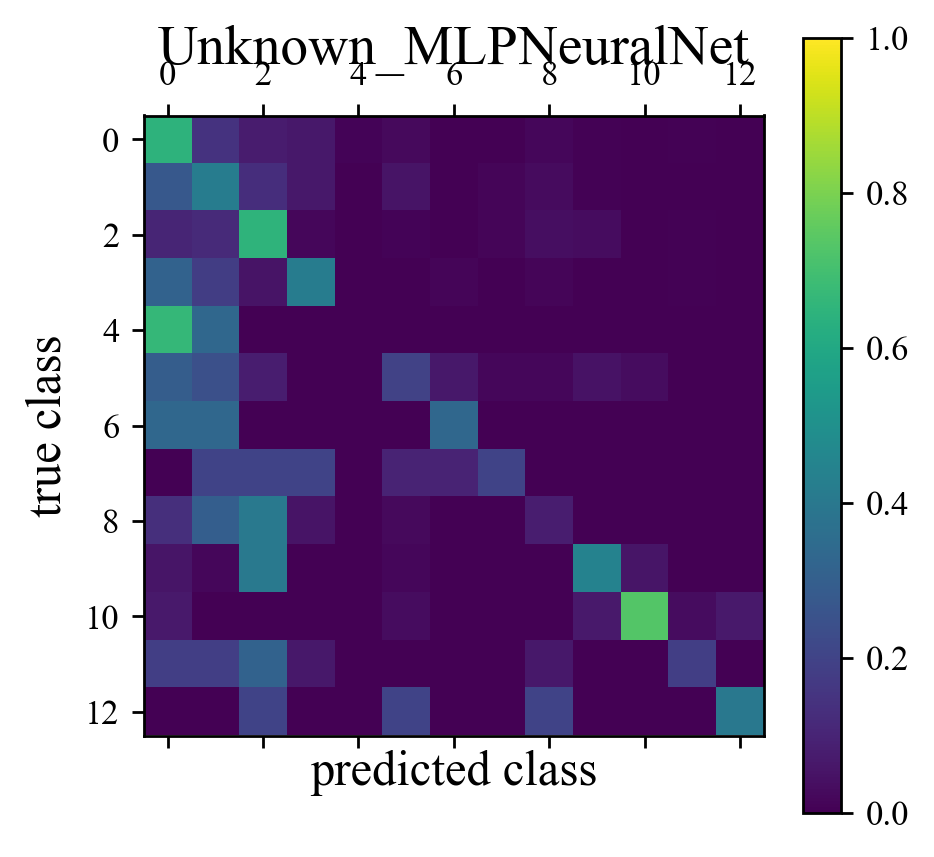
\includegraphics[width=0.3\textwidth]{./fig/Unknown_MLPNeuralNet_cm.png}
% 		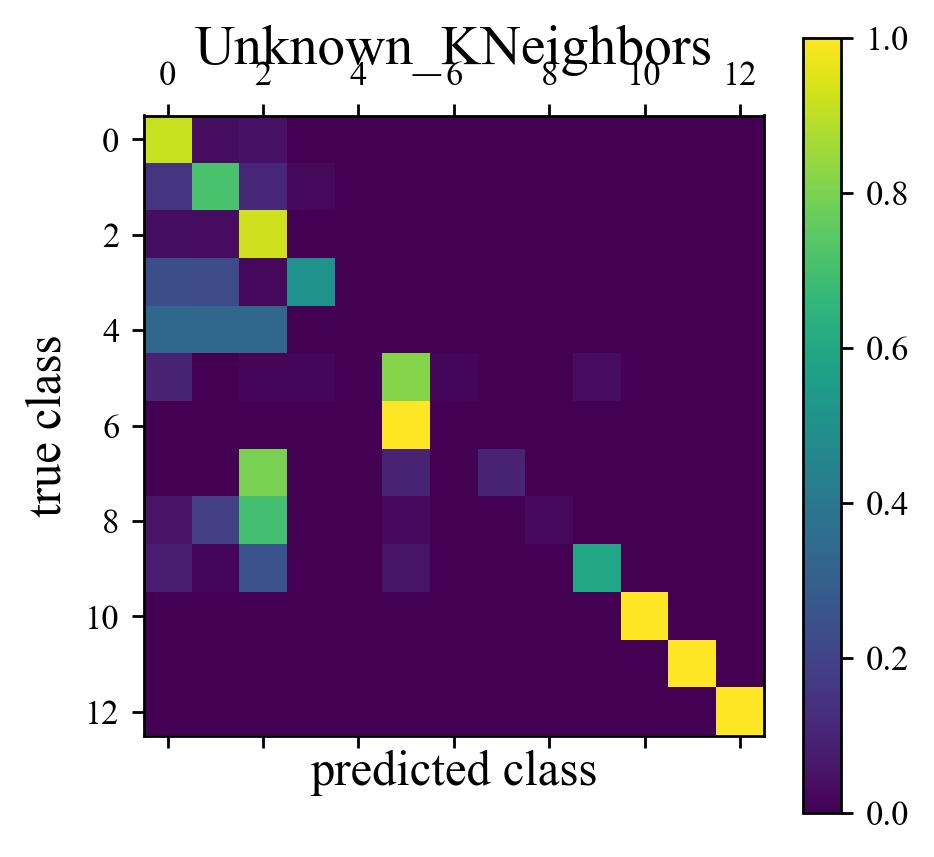
\includegraphics[width=0.3\textwidth]{./fig/Unknown_KNeighbors_cm.png}
% 		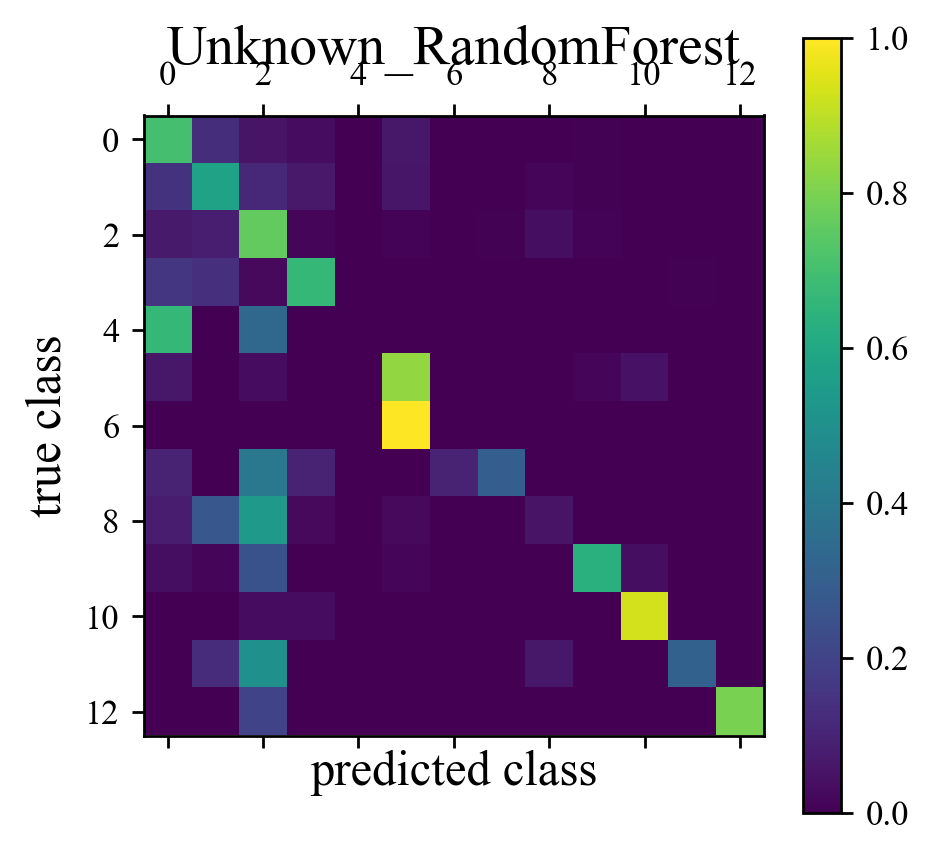
\includegraphics[width=0.3\textwidth]{./fig/Unknown_RandomForest_cm.png}
% 		\caption{}
% 		\label{fig:unknown_cm}
% 	\end{center}
% \end{figure*}
